% Provenance (never printed): see sources/outline_sources.md (Year 2: ancient massifs,
% Caledonian and Variscan belts; the Wilson cycle; supercontinents). Caledonian phases after
% McKerrow, Mac Niocaill and Dewey (2000) and Schiffer et al. (2020); the Wilson cycle after
% Chenin et al. (2018) and Schiffer et al. (2020); the Variscan belt after Faure (2024);
% supercontinents after Nance (2022); Siccar Point after the IUGS Geoheritage description.
% Model ocean and supercontinent chart from figdata/bachelor-2/wilson.py. Exercise and problem
% values in the Book 4 scratch calculator calc/ch15.py.
\chapter{Macizos antiguos y ciclo de Wilson}\label{ch:b2:wilson-cycle}

En la costa del sureste de Escocia, en Siccar Point, capas grises de arenisca se yerguen verticales
bajo una cubierta de arenisca roja que buza suavemente hacia el mar. Las capas grises se depositaron en
un océano a comienzos del Silúrico, y después se plegaron y adquirieron esquistosidad cuando ese océano se cerró; fueron desgastadas
hasta una superficie irregular; en el Devónico Superior unas gravas rojas las enterraron, y una segunda orogenia,
más suave, inclinó a su vez las capas rojas. Un solo acantilado registra un océano que ha
desaparecido, una cordillera que ya no existe y la siguiente. Este capítulo lee registros así,
los reúne en un ciclo que siguen las cuencas oceánicas, y da un paso atrás hacia el ritmo más largo de
todos, el ensamblaje y la fragmentación de los \omterm{def:b2:wilson-cycle:supercontinent}{supercontinentes}.
% ledger: iugs:siccar-orogenies, iugs:siccar-point

\begin{recall}
\textbf{De los volúmenes escolares}: Pangea y su fragmentación, los \omterm{def:b2:wilson-cycle:supercontinent}{supercontinentes}; las discordancias;
la tasa de denudación, el rebote isostático y el decrecimiento exponencial de una cordillera desgastada
por sus ríos. \textbf{Del volumen de primer año}: los rifts continentales, los márgenes pasivos y
las dorsales oceánicas, las velocidades de expansión total y semiexpansión; la subducción y los márgenes activos.
\textbf{Del \cref{ch:b2:crustal-melting} al \cref{ch:b2:himalaya-andes}}: las \omterm{def:b2:crustal-melting:migmatite}{migmatitas} y los
granitos; el \omterm{def:b2:alpine-orogen:orogen}{orógeno}, la \omterm{def:b2:alpine-orogen:ophiolite}{ofiolita}, la sutura, el \omterm{def:b2:alpine-orogen:nappes}{manto de corrimiento}, el \omterm{def:b2:alpine-orogen:foreland}{flysch} y la \omterm{def:b2:alpine-orogen:foreland}{molasa}, la \omterm{def:b2:alpine-orogen:foreland}{cuenca de antepaís}; los \omterm{def:b2:himalaya-andes:types}{orógenos de colisión}
y de tipo andino; el \omterm{def:b2:himalaya-andes:thickening}{engrosamiento cortical}, el espesor de Airy y el \omterm{def:b2:himalaya-andes:collapse}{colapso gravitacional}.
\end{recall}

\begin{omfigure}
\centering
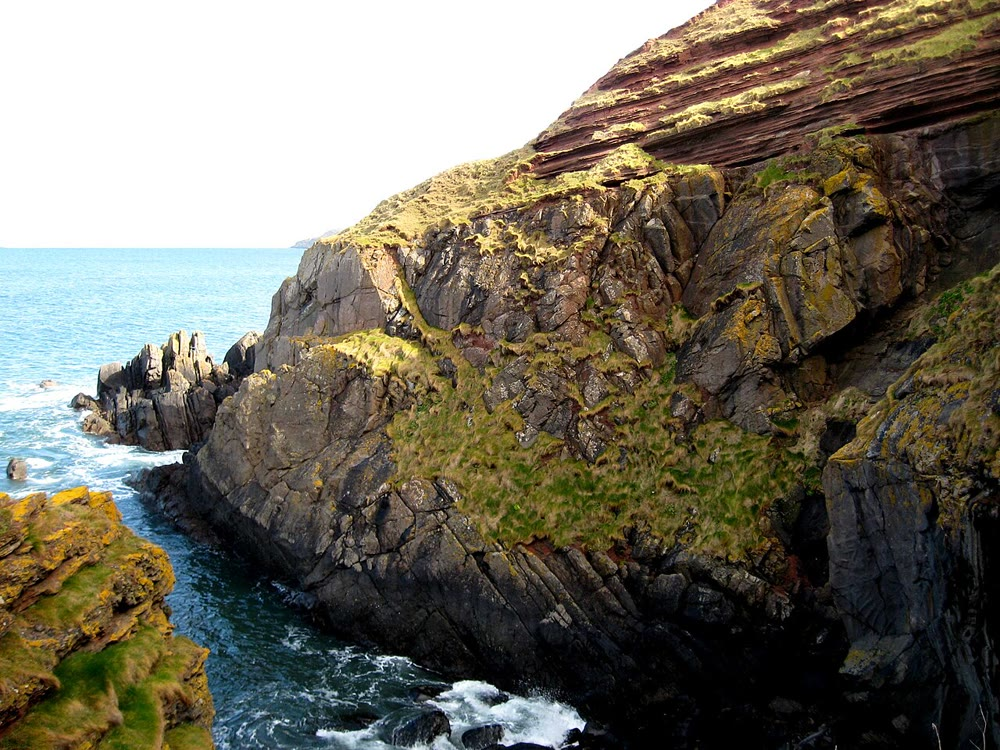
\includegraphics[width=0.64\linewidth]{images/book4/b2-15-siccar-point.jpg}
\par\smallskip{\small Siccar Point, al sureste de la punta: capas casi verticales de grauvaca gris
silúrica, plegadas en la orogenia caledoniana, bajo capas rojas suavemente inclinadas del
Devónico Superior. Fotografía de dave souza, 2008, CC BY-SA 4.0.}
\end{omfigure}
% ledger: iugs:siccar-orogenies

\section{Cordilleras desgastadas hasta sus raíces}\label{sec:b2:wilson-cycle:old}

Europa occidental y el este de Norteamérica están atravesados por cordilleras mucho más antiguas que los
Alpes. Sus cumbres han desaparecido, pero sus rocas permanecen. Tres de ellas nos interesan aquí.

La cordillera \emph{caledoniana} va de Noruega, por Escocia e Irlanda, hasta Terranova y
los Apalaches septentrionales, y sigue por el este de Groenlandia y Svalbard. Es el registro de un
océano, el Iapetus, que se extendía a comienzos del Paleozoico entre Laurentia, antecesora de Norteamérica
y Groenlandia, al noroeste, y Báltica y Avalonia al sureste y al este.
Sus márgenes se habían separado por rifting hace unos 600 millones de años; su cierre, del Cámbrico al
Devónico, produjo toda una serie de colisiones, de modo que la orogenia caledoniana abarca unos
200 millones de años. El término designa un lugar y un océano, no una edad.
% ledger: mckerrow00:caledonian, schiffer20:caledonides

La cordillera \emph{varisca}, llamada herciniana en los textos antiguos, atraviesa Europa desde el suroeste de
Inglaterra y Bélgica, por Francia e Iberia, hasta Europa central; la cordillera \emph{apalachiana} del
este de Norteamérica es su gemela occidental. Juntas registran el cierre de los océanos
entre el continente meridional, Gondwana, y el septentrional, que acababa de soldarse en
las colisiones caledonianas. Su última colisión, en el Carbonífero Superior y el Pérmico, dejó
un cinturón plegado que discurre de este a oeste por el sur de Europa y de nordeste a suroeste entre
el este de Norteamérica y el noroeste de África, y con él el \omterm{def:b2:wilson-cycle:supercontinent}{supercontinente} Pangea.
% ledger: schiffer20:variscan, faure24:variscan

¿Cómo se reconoce una cordillera que lleva trescientos millones de años erosionándose?
No por su relieve, que ha desaparecido. Se buscan sus partes, cada una de las cuales han encontrado ya los capítulos
anteriores:
\begin{itemize}
\item \emph{suturas} jalonadas de \emph{\omterm{def:b2:alpine-orogen:ophiolite}{ofiolitas}}, láminas del fondo del océano que se cerró;
\item franjas de \emph{rocas metamórficas}, a menudo de alto grado, las raíces de la corteza engrosada,
hoy en superficie porque los kilómetros que tenían encima se erosionaron;
\item \emph{granitos} y \emph{\omterm{def:b2:crustal-melting:migmatite}{migmatitas}}, productos de la fusión cortical que traen consigo
el engrosamiento y el calentamiento;
\item sedimentos del océano que se cierra y de la cordillera: \emph{\omterm{def:b2:alpine-orogen:foreland}{flysch}} vertido en cuencas profundas
durante la convergencia, \emph{\omterm{def:b2:alpine-orogen:foreland}{molasa}} vertida en \omterm{def:b2:alpine-orogen:foreland}{cuencas de antepaís} e intramontañosas;
\item \emph{discordancias angulares}, donde capas más jóvenes descansan sobre capas que se plegaron y
erosionaron antes que ellas, y fechan la deformación entre ambas.
\end{itemize}

\begin{definition}[Penillanura]\label{def:b2:wilson-cycle:peneplain}
Una \emph{penillanura}\index{penillanura} es una superficie terrestre de relieve bajo, próxima al nivel de base de
la erosión, labrada sobre rocas de distinta dureza y estructura por la larga erosión de un antiguo
relieve.
\end{definition}

La cordillera varisca es un \omterm{def:b2:alpine-orogen:orogen}{orógeno} caliente. En los Alpes del \cref{ch:b2:alpine-orogen}, las rocas
siguieron gradientes metamórficos de unos \qty{8}{\celsius} por kilómetro; en la cordillera varisca,
de unos \qty{30}{\celsius} por kilómetro. Su corteza fundió ampliamente: en el Macizo Central francés
y el Macizo Armoricano se formaron \omterm{def:b2:crustal-melting:migmatite}{migmatitas} hace entre unos 330 y 325 millones de años, y
granitos intruyeron en ellas. Esa fusión es la principal diferencia con los Alpes occidentales. Al terminar la
colisión, la corteza engrosada se adelgazó por extensión, las rocas metamórficas ascendieron
a lo largo de \omterm{def:b2:alpine-orogen:decollement}{despegues} y se abrieron cuencas intramontañosas; después la erosión niveló la cordillera hasta una
\omterm{def:b2:wilson-cycle:peneplain}{penillanura} pérmica y triásica sobre la que se depositaron los sedimentos del ciclo siguiente.
% ledger: faure24:variscan

\begin{omfigure}
\centering\small
\begin{tabular}{>{\raggedright\arraybackslash}p{0.2\linewidth}|>{\raggedright\arraybackslash}p{0.17\linewidth}|>{\raggedright\arraybackslash}p{0.52\linewidth}}
fase & edad & qué colisionó \\ \hline
Penobscótica & 490--485 Ma & un arco insular cabalgó sobre el margen avalónico \\
Grampiana, Tacónica & 480--455 Ma & arcos insulares contra Laurentia (Escocia; los Apalaches septentrionales) \\
Shelveiana & comienzos del Ordovícico Superior & Avalonia contra Báltica; se cierra el mar de Tornquist \\
Escandiana & 425--400 Ma & Báltica contra Laurentia; los grandes \omterm{def:b2:alpine-orogen:nappes}{mantos de corrimiento} de Escandinavia \\
Acádica & Devónico Inferior & \omterm{def:b2:wilson-cycle:terrane}{terranes} procedentes de Gondwana contra el nuevo continente; Iapetus cerrado \\
\end{tabular}
\par\smallskip{\small Las principales fases de la orogenia caledoniana. Las primeras fases son
colisiones de arcos con arcos o con continentes, y las últimas, colisiones de continentes; la mayoría de las
fases empezaron en momentos distintos en lugares distintos.}
\end{omfigure}
% ledger: mckerrow00:phases, schiffer20:caledonides

La tabla caledoniana anterior muestra la otra marca de las cordilleras antiguas: son compuestas. Antes de que
los dos continentes se encontraran, arcos y bloques menores fueron llegando uno a uno y soldándose.

\begin{definition}[Terrane; microcontinente]\label{def:b2:wilson-cycle:terrane}
Un \emph{terrane}\index{terrane} es un bloque de corteza limitado por fallas cuya historia geológica
difiere de la de sus vecinos, llevado a su posición actual por el movimiento de las placas; puede
ser un arco insular, una meseta oceánica, una lámina de fondo oceánico o un fragmento de continente. Un
\emph{microcontinente}\index{microcontinente} es un bloque de corteza continental, más pequeño que un
continente, separado de los continentes por corteza oceánica.
\end{definition}

Avalonia fue un bloque así: una franja de corteza que se separó del margen de Gondwana, abrió el océano
Rheico tras ella en el Ordovícico, atravesó el Iapetus y se acopló a Báltica y después a
Laurentia. Armórica y Saxoturingia, hoy en Francia y Alemania, la siguieron a su vez; sus
suturas, marcadas por \omterm{def:b2:alpine-orogen:ophiolite}{ofiolitas}, dividen la cordillera varisca en zonas que van de un antepaís septentrional
en el antiguo continente del norte a un antepaís meridional en Gondwana.
% ledger: schiffer20:caledonides, schiffer20:variscan, faure24:variscan

\begin{omfigure}
\centering
\begin{tikzpicture}[x=0.5cm, y=0.5cm, font=\scriptsize]
\tikzset{cont/.style={fill=orange!25, draw=black!60, line width=0.4pt},
  terr/.style={fill=orange!45, draw=black!60, line width=0.4pt},
  ocn/.style={font=\scriptsize\itshape, text=blue!50!black},
  belt/.style={pattern=north east lines, pattern color=red!60!black, draw=red!60!black}}
% panel A
\begin{scope}
\fill[blue!6] (0,0) rectangle (9,8);
\draw[cont] (0.3,4.2) -- (3.0,4.0) -- (3.4,7.7) -- (0.3,7.7) -- cycle;
\node[align=center] at (1.7,6.0) {Lau-\\rentia};
\draw[cont] (6.0,5.4) -- (8.7,5.0) -- (8.7,7.7) -- (6.4,7.7) -- cycle;
\node at (7.4,6.6) {Báltica};
\draw[cont] (0.3,0.3) -- (8.7,0.3) -- (8.7,1.6) -- (0.3,1.9) -- cycle;
\node at (4.5,0.95) {Gondwana};
\draw[terr] (3.8,2.4) -- (6.6,2.2) -- (6.6,2.9) -- (3.8,3.1) -- cycle;
\node at (5.2,2.65) {Avalonia};
\node[ocn] at (4.6,5.4) {Iapetus};
\node[ocn] at (7.7,2.55) {Rheico};
\node[anchor=north west, font=\small\bfseries] at (0.1,8.9) {A: hacia 480 Ma};
\end{scope}
% panel B
\begin{scope}[xshift=5.0cm]
\fill[blue!6] (0,0) rectangle (9,8);
\draw[cont] (0.3,3.6) -- (3.0,3.4) -- (3.4,7.7) -- (0.3,7.7) -- cycle;
\draw[cont] (3.0,3.4) -- (3.4,7.7) -- (8.7,7.7) -- (8.7,4.4) -- (5.2,4.6) -- (5.0,3.4) -- cycle;
\draw[terr] (3.0,3.4) -- (5.0,3.4) -- (5.2,4.6) -- (8.7,4.4) -- (8.7,3.6) -- (3.0,2.8) -- cycle;
\draw[red!60!black, line width=1.2pt] (3.0,3.4) -- (3.4,7.7);
\draw[red!60!black, line width=1.2pt] (5.0,3.4) -- (5.2,4.6) -- (8.7,4.4);
\node[align=center] at (1.6,5.6) {Lau-\\rentia};
\node at (6.6,5.7) {Báltica};
\node at (6.4,3.75) {Avalonia};
\node at (6.0,7.1) {\textbf{Laurusia}};
\draw[cont] (0.3,0.3) -- (8.7,0.3) -- (8.7,1.3) -- (0.3,1.5) -- cycle;
\node at (4.5,0.8) {Gondwana};
\draw[terr] (2.2,1.9) -- (3.6,1.9) -- (3.6,2.3) -- (2.2,2.3) -- cycle;
\draw[terr] (5.0,1.8) -- (6.6,1.8) -- (6.6,2.2) -- (5.0,2.2) -- cycle;
\node[ocn] at (7.7,2.3) {Rheico};
\node[anchor=north west, font=\small\bfseries] at (0.1,8.9) {B: hacia 420 Ma};
\end{scope}
% panel C
\begin{scope}[xshift=10.0cm]
\fill[blue!6] (0,0) rectangle (9,8);
\draw[cont] (0.3,3.0) -- (8.7,3.0) -- (8.7,7.7) -- (0.3,7.7) -- cycle;
\draw[cont] (0.3,0.3) -- (8.7,0.3) -- (8.7,3.0) -- (0.3,3.0) -- cycle;
\fill[belt] (0.3,2.5) -- (8.7,2.5) -- (8.7,3.5) -- (0.3,3.5) -- cycle;
\node[fill=orange!25, inner sep=1pt] at (4.5,5.6) {Laurusia};
\node[fill=orange!25, inner sep=1pt] at (4.5,1.3) {Gondwana};
\node[fill=white, fill opacity=0.85, text opacity=1, inner sep=1pt, align=center] at (4.5,3.0)
  {cordillera\\varisca--apalachiana};
\node[ocn] at (7.6,0.7) {};
\node[anchor=north west, font=\small\bfseries] at (0.1,8.9) {C: hacia 300 Ma, Pangea};
\end{scope}
\end{tikzpicture}
\par\smallskip{\small Tres momentos del cierre de los océanos Iapetus y Rheico, en un
esbozo esquemático sin proyección cartográfica ni escala: las posiciones, los tamaños y las formas son solo
topológicos. A: Avalonia se ha separado de Gondwana y el océano Rheico se abre tras ella. B: el Iapetus se ha
cerrado; Laurentia, Báltica y Avalonia forman Laurusia, a lo largo de suturas caledonianas (líneas rojas);
bloques menores atraviesan el océano Rheico. C: Gondwana se ha encontrado con Laurusia a lo largo de la
cordillera varisca--apalachiana (rayada).}
\end{omfigure}
% ledger: mckerrow00:caledonian, mckerrow00:phases, schiffer20:caledonides, schiffer20:variscan, faure24:variscan

\section{El ciclo de Wilson}\label{sec:b2:wilson-cycle:cycle}

En 1966 J. Tuzo Wilson se preguntó si el Atlántico se había cerrado y después
vuelto a abrir. Los fósiles del Paleozoico inferior y medio le indicaban que un océano amplio había
separado entonces las faunas de Norteamérica de las de Europa occidental, un océano que ya no
existía desde finales del Paleozoico hasta mediados del Mesozoico. El Atlántico moderno se había abierto
casi donde aquel océano más antiguo, el Iapetus, se había cerrado.
% ledger: schiffer20:wilson, chenin18:cycle

\begin{definition}[Ciclo de Wilson]\label{def:b2:wilson-cycle:wilson}
El \emph{ciclo de Wilson}\index{ciclo de Wilson} es la sucesión de etapas por las que una
cuenca oceánica se abre y vuelve a cerrarse entre márgenes continentales: rifting continental,
ruptura y expansión del fondo oceánico, un océano que se ensancha con márgenes pasivos, el inicio de la
subducción, el estrechamiento y cierre del océano, la colisión continental, y el colapso
y la erosión de la cordillera, tras lo cual el continente soldado puede volver a abrirse por rift a lo largo de la misma zona.
\end{definition}

La figura siguiente recorre las etapas. Son las de los capítulos anteriores puestas en orden:
los rifts y márgenes pasivos del volumen de primer año, los márgenes activos y sus arcos, las
colisiones alpina e himalaya, el \omterm{def:b2:himalaya-andes:collapse}{colapso gravitacional} del Tíbet, el lento desgaste
de las cordilleras antiguas.

\begin{omfigure}
\centering
\begin{tikzpicture}[x=0.38cm, y=0.38cm, font=\scriptsize]
\tikzset{crust/.style={fill=orange!25, draw=black!60, line width=0.3pt},
  ocrust/.style={fill=gray!45, draw=black!60, line width=0.3pt},
  sea/.style={fill=blue!8},
  ttl/.style={anchor=west, font=\scriptsize\bfseries}}
% 1 continent
\begin{scope}
\draw[crust] (0,0) -- (16,0) -- (16,2) -- (0,2) -- cycle;
\node[ttl] at (0,3.1) {1\enspace un continente};
\end{scope}
% 2 rift
\begin{scope}[xshift=7.2cm]
\draw[crust] (0,0) -- (7,0) -- (7,2) -- (6.2,2) -- (5.4,1.0) -- (0,2) -- cycle;
\draw[crust] (9,0) -- (16,0) -- (16,2) -- (10.6,1.0) -- (9.8,2) -- (9,2) -- cycle;
\fill[red!50] (7,0) -- (9,0) -- (8.6,1.2) -- (7.4,1.2) -- cycle;
\draw[thick] (6.2,2) -- (7,0.4); \draw[thick] (9.8,2) -- (9,0.4);
\node[ttl] at (0,3.1) {2\enspace rift};
\end{scope}
% 3 young ocean
\begin{scope}[yshift=-2.4cm]
\fill[sea] (5,2) -- (11,2) -- (11,0.6) -- (5,0.6) -- cycle;
\draw[crust] (0,0) -- (5,0) -- (6.2,0.5) -- (5,2) -- (0,2) -- cycle;
\draw[crust] (16,0) -- (11,0) -- (9.8,0.5) -- (11,2) -- (16,2) -- cycle;
\draw[ocrust] (6.2,0.5) -- (9.8,0.5) -- (9.8,0) -- (6.2,0) -- cycle;
\draw[red!70!black, thick] (8,0.5) -- (8,1.0);
\node[ttl] at (0,3.1) {3\enspace un océano joven};
\end{scope}
% 4 wide ocean
\begin{scope}[xshift=7.2cm, yshift=-2.4cm]
\fill[sea] (2.5,2) -- (13.5,2) -- (13.5,0.4) -- (2.5,0.4) -- cycle;
\draw[crust] (0,0) -- (2.5,0) -- (3.4,0.4) -- (2.5,2) -- (0,2) -- cycle;
\draw[crust] (16,0) -- (13.5,0) -- (12.6,0.4) -- (13.5,2) -- (16,2) -- cycle;
\draw[ocrust] (3.4,0.4) -- (12.6,0.4) -- (12.6,-0.4) -- (3.4,-0.4) -- cycle;
\draw[red!70!black, thick] (8,0.4) -- (8,0.9);
\node[anchor=north] at (3,-0.1) {pasivo};
\node[anchor=north] at (13,-0.1) {pasivo};
\node[ttl] at (0,3.1) {4\enspace un océano amplio};
\end{scope}
% 5 subduction begins
\begin{scope}[yshift=-4.8cm]
\fill[sea] (2.5,2) -- (13.5,2) -- (13.5,0.4) -- (2.5,0.4) -- cycle;
\draw[crust] (0,0) -- (2.5,0) -- (3.4,0.4) -- (2.5,2) -- (0,2) -- cycle;
\draw[crust] (16,-0.4) -- (13.3,-0.4) -- (12.6,0.4) -- (13.5,2) -- (16,2) -- cycle;
\draw[ocrust] (3.4,0.4) -- (12.6,0.4) -- (11.6,-1.6) -- (3.4,-0.4) -- cycle;
\fill[red!60!black] (14.2,2) -- (14.6,2.7) -- (15.0,2) -- cycle;
\draw[red!70!black, thick] (7,0.4) -- (7,0.9);
\node[anchor=north] at (13.5,-0.5) {fosa};
\node[ttl] at (0,3.1) {5\enspace empieza la subducción};
\end{scope}
% 6 ocean closes
\begin{scope}[xshift=7.2cm, yshift=-4.8cm]
\fill[sea] (5.5,2) -- (10.5,2) -- (10.5,0.4) -- (5.5,0.4) -- cycle;
\draw[crust] (0,0) -- (5.5,0) -- (6.4,0.4) -- (5.5,2) -- (0,2) -- cycle;
\draw[crust] (16,-0.4) -- (11.3,-0.4) -- (10.6,0.4) -- (11.5,2.4) -- (16,2.4) -- cycle;
\draw[ocrust] (6.4,0.4) -- (10.6,0.4) -- (9.4,-1.8) -- (6.4,-0.4) -- cycle;
\fill[red!60!black] (12.4,2.4) -- (12.8,3.1) -- (13.2,2.4) -- cycle;
\node[anchor=north west] at (11.6,-0.5) {arco, fosa};
\node[ttl] at (0,3.1) {6\enspace el océano se cierra};
\end{scope}
% 7 collision
\begin{scope}[yshift=-7.2cm]
\draw[crust] (0,0) -- (16,0) -- (16,2) -- (10,2) -- (8.6,3.6) -- (7.4,3.4) -- (6,2) -- (0,2) -- cycle;
\fill[crust] (5.6,0) -- (10.4,0) -- (9.6,-1.6) -- (6.4,-1.6) -- cycle;
\draw[black!60, line width=0.3pt] (5.6,0) -- (6.4,-1.6) -- (9.6,-1.6) -- (10.4,0);
\draw[red!60!black, line width=1pt] (8.6,3.6) -- (7.6,-1.6);
\node[anchor=west, text=red!60!black] at (9.0,3.5) {sutura};
\node[ttl] at (0,3.1) {7\enspace colisión};
\end{scope}
% 8 worn flat
\begin{scope}[xshift=7.2cm, yshift=-7.2cm]
\draw[crust] (0,0) -- (16,0) -- (16,2) -- (0,2) -- cycle;
\draw[red!60!black, line width=1pt] (8.4,2) -- (7.6,0);
\fill[pink!60!red!40] (6.0,1.0) ellipse (0.7 and 0.4);
\node[anchor=north] at (8,-0.1) {penillanura sobre la antigua raíz};
\node[ttl] at (0,3.1) {8\enspace una cordillera arrasada; puede seguir un rift};
\end{scope}
\end{tikzpicture}
\par\smallskip{\small Las etapas del \omterm{def:b2:wilson-cycle:wilson}{ciclo de Wilson}, en cortes esquemáticos (sin escala):
corteza continental en naranja, corteza oceánica en gris, la dorsal en rojo, los volcanes del arco como
triángulos; en el último panel, la sutura y un granito permanecen en una corteza de espesor normal.}
\end{omfigure}
% ledger: chenin18:cycle, schiffer20:wilson

\subsection{¿Qué anchura, cuánto tiempo?}

Un océano crece por expansión del fondo oceánico en su dorsal y se reduce por subducción en sus fosas.
Una contabilidad sencilla da su anchura.

\begin{proposition}[Anchura de un océano a lo largo de un ciclo]\label{prop:b2:wilson-cycle:width}
Sea un océano que se abre en el instante $t_0$ y se ensancha a la velocidad de expansión total $V_s$ de su dorsal, hasta que
una zona de subducción empieza en uno de sus márgenes en el instante $t_1$ y consume fondo oceánico a la velocidad $V_c$
respecto de ese margen, con $V_c > V_s$, mientras la dorsal sigue en expansión. Su anchura es
\[
  W(t) = V_s\,(t - t_0) \quad (t_0 \le t \le t_1), \qquad
  W(t) = V_s\,(t_1 - t_0) - (V_c - V_s)\,(t - t_1) \quad (t \ge t_1),
\]
máxima en $t_1$, y el océano se cierra un tiempo $V_s(t_1 - t_0)/(V_c - V_s)$ después del inicio de la
subducción. Con una expansión simétrica, la dorsal se desplaza hacia la fosa a $V_c - V_s/2$.
\end{proposition}

\begin{proof}
Manténgase fijo el margen con la fosa. Antes de $t_1$ los dos márgenes se separan a la velocidad de expansión
total $V_s$, de modo que la anchura crece a $V_s$ desde cero. Después de $t_1$ la placa entre la
fosa y la dorsal se desplaza hacia la fosa a $V_c$; la dorsal añade $V_s$ a la distancia
entre esa placa y la placa opuesta, de modo que el margen opuesto se desplaza hacia la fosa a $V_c - V_s$,
la velocidad a la que disminuye la anchura. La anchura se anula al cabo de $V_s(t_1 - t_0)/(V_c -
V_s)$. Con una expansión simétrica, la dorsal se mueve a la media de las velocidades de las placas situadas a
uno y otro lado, $(V_c + (V_c - V_s))/2 = V_c - V_s/2$.
\end{proof}

La figura siguiente aplica esta contabilidad a un océano modelo de tipo Iapetus: expansión desde
\qty{570}{Ma} a \qty{30}{mm} al año, subducción desde \qty{490}{Ma} que consume \qty{60}{mm} al
año. Las velocidades son hipótesis, valores redondos del orden de los que se miden hoy en los océanos; el
Iapetus real no fue tan sencillo ni se conoce tan bien. El océano modelo alcanza \qty{2400}{km}
y se cierra a \qty{410}{Ma}, dentro del intervalo de la colisión escandiana.
% values (wilson.py): max_width_km 2400, closure_Ma 410; ledger: mckerrow00:caledonian, schiffer20:caledonides

\begin{omfigure}
\centering
% figdata/bachelor-2/wilson.py part ocean (model values: assumptions)
\begin{tikzpicture}
\begin{axis}[width=0.8\linewidth, height=5.0cm, x dir=reverse, xmin=360, xmax=600, ymin=0,
  ymax=3300, ytick={0,1000,2000,3000}, xlabel={edad (\unit{Ma})}, ylabel={anchura del océano (\unit{km})},
  tick label style={font=\scriptsize}, label style={font=\small}, xtick={600,560,...,360}]
\addplot[omThm, line width=1.2pt] table[x=t_Ma, y=width_km] {figdata/out/bachelor-2-wilson-ocean.dat};
\draw[dashed, black!50] (axis cs:490,0) -- (axis cs:490,2400);
\draw[dashed, black!50] (axis cs:570,0) -- (axis cs:570,2750);
\draw[dashed, black!50] (axis cs:410,0) -- (axis cs:410,2750);
\node[font=\scriptsize, anchor=south west] at (axis cs:570,2750) {empieza la expansión};
\node[font=\scriptsize, anchor=south west] at (axis cs:488,2400) {empieza la subducción};
\node[font=\scriptsize, anchor=south] at (axis cs:410,2750) {colisión};
\node[font=\scriptsize, anchor=west] at (axis cs:540,600) {apertura a $V_s$};
\node[font=\scriptsize, anchor=south west, align=left] at (axis cs:446,1150) {cierre\\a $V_c - V_s$};
\end{axis}
\end{tikzpicture}
\par\smallskip{\small Anchura de un océano modelo a lo largo de un \omterm{def:b2:wilson-cycle:wilson}{ciclo de Wilson}, según la
\cref{prop:b2:wilson-cycle:width} con $V_s = \qty{30}{mm}$ al año desde \qty{570}{Ma} y $V_c
= \qty{60}{mm}$ al año desde \qty{490}{Ma}. El tiempo avanza de izquierda a derecha.}
\end{omfigure}

\subsection{Abrirse donde se cerró}

La idea de Wilson descansa en otra, mecánica: una cordillera antigua es una zona débil, y un continente sometido
a estiramiento tiende a romperse a lo largo de sus zonas débiles más que a través de su interior
resistente y estable.

\begin{definition}[Reactivación estructural]\label{def:b2:wilson-cycle:reactivation}
La \emph{reactivación estructural}\index{reactivación estructural} de una estructura preexistente
(una falla, una zona de cizalla, una sutura, un contacto litológico) es la nueva concentración de la
deformación a lo largo de ella, bajo un campo de esfuerzos posterior que puede diferir del que la formó.
\end{definition}

El Atlántico Norte es el caso de prueba, y solo lo supera en parte. En el Atlántico Central el
joven océano sigue de cerca los Apalaches. Entre Escandinavia y Groenlandia la ruptura
sigue a grandes rasgos la cordillera caledoniana. Más al sur no: la sutura del Iapetus sigue atravesando
el norte de Inglaterra y el centro de Irlanda, y el Atlántico se abrió al oeste de ella, dejando
fragmentos de la antigua corteza de Laurentia en el margen noroccidental de Europa, en torno a Rockall y Hatton.
Más al noroeste, el mar de Labrador y la bahía de Baffin cortan directamente cratones y
cordilleras más antiguos. Las estructuras antiguas guían los rifts posteriores, pero no siempre: una debilidad que se ha enfriado durante más
de 30 a 50 millones de años puede haberse vuelto resistente, y un nuevo rift puede seguir la fábrica más profunda
del manto en lugar de la sutura cortical. El \omterm{def:b2:wilson-cycle:wilson}{ciclo de Wilson} es una guía, no una ley.
% ledger: schiffer20:wilson, schiffer20:reactivation

No todos los ciclos abren un océano amplio. Muchos \omterm{def:b2:alpine-orogen:orogen}{orógenos} cierran océanos embrionarios, rifts que apenas habían
empezado a expandirse, de menos de unos \qty{500}{km} de anchura: los Alpes, los Pirineos, la mayor parte de la
cordillera varisca de Europa occidental. Otros cierran océanos amplios y maduros, como hicieron las Caledónides
escandinavas. La diferencia se nota al final. Una cordillera que cerró un océano amplio tuvo un
arco de larga vida, que vació el manto subyacente de su parte fusible; su colapso fue pobre en
\omterm{def:b2:magma-emplacement:magma}{magma}, como en las Caledónides. Una cordillera que cerró una cuenca estrecha se asienta sobre un \omterm{def:b2:mantle-melting:fertility}{manto fértil}; su
colapso puede ser rico en \omterm{def:b2:magma-emplacement:magma}{magma}, como en la cordillera varisca, donde el Moho es hoy plano y la
corteza inferior está estratificada, lo que se interpreta como basalto subplacado bajo la corteza o como corteza inferior cizallada
en caliente. En unas pocas decenas de millones de años las anomalías
térmicas de una cordillera se desvanecen; sus estructuras permanecen.
% ledger: chenin18:cycle

\section{Los supercontinentes}\label{sec:b2:wilson-cycle:supercontinents}

\begin{definition}[Supercontinente; ciclo de los supercontinentes]\label{def:b2:wilson-cycle:supercontinent}
Un \emph{supercontinente}\index{supercontinente} es una masa de tierra que reúne la mayor parte de la
corteza continental de la Tierra en un solo bloque. El \emph{ciclo de los supercontinentes}\index{ciclo de los supercontinentes} es
el ensamblaje episódico de los continentes en un supercontinente y su posterior
fragmentación, repetidos a lo largo de la historia de la Tierra.
\end{definition}

Pangea, que Wegener reconstruyó y que describieron los volúmenes escolares, existió desde hace unos 325
hasta hace unos 200 millones de años. Se han propuesto \omterm{def:b2:wilson-cycle:supercontinent}{supercontinentes} anteriores: Pannotia, hace unos 620 a
580 millones de años, cuya existencia se discute; Rodinia, hace unos 950 a 800 millones de años;
Nuna, también llamado Columbia, hace unos 1.6 a 1.4 miles de millones de años; y, más dudosos, Kenorland,
hace unos 2.7 a 2.5 miles de millones de años, y Ur, hace unos 3.0 miles de millones de años. Parecen haberse
ensamblado y fragmentado a intervalos de aproximadamente quinientos millones de años desde quizá finales del
Arcaico. El ciclo se ha relacionado con las edades de las orogenias, con los picos de edad de los
granitos y de los granos de circón que contienen, con el crecimiento de la corteza, con las grandes provincias
ígneas, con el nivel del mar y con el clima: el ensamblaje de un \omterm{def:b2:wilson-cycle:supercontinent}{supercontinente} tiende a coincidir
con un enfriamiento.
% ledger: nance22:supercontinents

\begin{omfigure}
\centering
% figdata/bachelor-2/wilson.py part supercontinents; ledger: nance22:supercontinents
\begin{tikzpicture}
\begin{axis}[width=0.86\linewidth, height=4.6cm, x dir=reverse, xmin=0, xmax=3300, ymin=-0.7,
  ymax=6.5, ytick=\empty, xlabel={edad (\unit{Ma})}, tick label style={font=\scriptsize},
  label style={font=\small}, xtick={0,500,...,3000}, axis y line*=left,
  % etiquetas: nodos explícitos (la tabla de figdata lleva los nombres en inglés)
  clip=false]
\addplot[only marks, mark=*, mark size=1.6pt, omThm,
  error bars/.cd, x dir=both, x explicit, error bar style={line width=3pt, omThm!60}, error mark=none]
  table[x=mid_Ma, y=row, x error=half_Ma] {figdata/out/bachelor-2-wilson-supercontinents.dat}; \foreach \x/\y/\n in {3000/0/Ur, 2600/1/Kenorland, 1500/2/Nuna-Columbia, 875/3/Rodinia, 600/4/Pannotia, 262.5/5/Pangea} {\edef\temp{\noexpand\node[font=\noexpand\scriptsize, anchor=south, yshift=2pt] at (axis cs:\x,\y) {\n};}\temp}
\end{axis}
\end{tikzpicture}
\par\smallskip{\small Los \omterm{def:b2:wilson-cycle:supercontinent}{supercontinentes} a lo largo de la historia de la Tierra, del ensamblaje a la fragmentación, según las
fechas de una revisión reciente: las barras abarcan los intervalos citados (Ur es una sola estimación), y los
puntos, sus puntos medios. Pannotia, Kenorland y Ur son discutidos. El tiempo avanza de izquierda a derecha.}
\end{omfigure}

¿Es el ciclo verdaderamente periódico? Los puntos medios de los intervalos del gráfico están separados por 400,
1100, 625, 275 y 337.5 millones de años: en promedio unos 550, pero con una dispersión de un factor
cuatro. «Aproximadamente quinientos millones de años» es una tendencia, no un reloj, y los \omterm{def:b2:wilson-cycle:supercontinent}{supercontinentes} más
antiguos descansan en pruebas escasas.
% values (wilson.py): spacings 400 1100 625 275 337.5, mean 547.5 Myr

\section{De las montañas a las llanuras}\label{sec:b2:wilson-cycle:erosion}

¿Qué convierte una cordillera como el Himalaya en las colinas bajas de Bretaña? El volumen de bachillerato
construyó un modelo: los ríos desgastan una cordillera a una velocidad proporcional a su altitud media, $kh$,
y cada metro retirado de la cima se recupera en parte por rebote isostático, de modo que solo
la fracción $f = (\rho_m - \rho_c)/\rho_m$ se pierde como altura. La altitud media
decrece entonces según
\[
  h(t) = h_0\,e^{-k f t} ,
\]
con la constante de tiempo $\tau = 1/(kf)$. En las grandes cuencas de latitudes medias, la tasa de denudación es
proporcional al relieve medio, y sin levantamiento el relieve caería a la décima parte de su
valor en unos 11 millones de años: $k = \ln 10/11 \approx 0.21$ por millón de años. Con las
densidades de 2700 y \qty{3300}{kg.m^{-3}}, $f = 0.18$ y $\tau \approx \qty{26}{Myr}$: una
cordillera de \qty{3}{km} de altura sigue teniendo \qty{1}{km} unos 30 millones de años después, y baja
de \qty{300}{m} al cabo de unos 60 millones de años.
% ledger: ahnert70:decay; values (wilson.py): k 0.20933 /Myr, f 0.18182, tau 26.275 Myr

El mismo rebote explica por qué las cordilleras antiguas dejan al descubierto sus raíces. Para devolver al nivel del mar una corteza engrosada de
$H$ a $T$, hay que erosionar todo el espesor adicional $T - H$, mientras que la altitud media
era solo $(T - H)f$: se retira unas 5.5 veces más roca que la altura de la
cordillera. Rocas que estaban a 20 o \qty{30}{km} de profundidad en la raíz llegan a la superficie: las
\omterm{def:b2:crustal-melting:migmatite}{migmatitas}, los granitos y los gneises de alto grado de los macizos antiguos, como los del Macizo
Central.
% ledger: ahnert70:decay

La cordillera varisca, cuyas últimas colisiones terminaron hace unos 290 millones de años, había quedado
nivelada en una \omterm{def:b2:wilson-cycle:peneplain}{penillanura} durante el Pérmico y el Triásico: dentro de los 60 millones de años aproximadamente
que da el modelo. El colapso puede acelerarlo: la extensión de una corteza engrosada, como en el
Tíbet actual, la adelgaza directamente, sin esperar a los ríos. Y en Siccar Point, gravas del Devónico Superior descansan sobre
capas silúricas plegadas en las colisiones caledonianas, sobre una antigua superficie terrestre que todavía conserva
cierto relieve entre las capas duras y las blandas.
% ledger: faure24:variscan, iugs:siccar-orogenies

\begin{inthefield}[Leer una discordancia angular]
Los geólogos que estudian una discordancia angular como la de Siccar Point empiezan midiendo la
orientación de las capas por debajo y por encima de la superficie, dirección y buzamiento, en muchos puntos. Buscan
la polaridad de las capas inferiores, por la granoclasificación o por las marcas de la base de las capas,
ya que las capas plegadas pueden estar invertidas. Examinan la propia superficie: su relieve, la
alteración bajo ella, los cantos de las rocas antiguas en el conglomerado que tiene encima. Después
datan: los fósiles más jóvenes de abajo dan la edad antes de la cual no puede haber ocurrido el plegamiento,
y los fósiles más antiguos de arriba, la edad antes de la cual ya había ocurrido y la tierra se había
desgastado. El intervalo entre ambas acota la orogenia. En Siccar Point las capas inferiores son del Silúrico
inferior y las superiores del Devónico Superior, y el plegamiento, el levantamiento y la erosión caledonianos caben
entre ambas; la suave inclinación de las capas superiores es más reciente aún, varisca.
\end{inthefield}
% ledger: iugs:siccar-orogenies, ics:base.Silurian, ics:base.Devonian, ics:base.Carboniferous

\section*{Ejercicios}\label{sec:b2:wilson-cycle:exercises}

Datos para los ejercicios: $g = \qty{9.8}{m.s^{-2}}$; densidades de la corteza y del manto
\qty{2700}{kg.m^{-3}} y \qty{3300}{kg.m^{-3}}; corteza normal $H = \qty{35}{km}$; edades de las
bases del Silúrico, el Devónico y el Carbonífero 443.1, 419.6 y \qty{358.9}{Ma}, y de la del
Triásico \qty{251.9}{Ma}.

\begin{exercise}[$\star$]\label{exo:b2:wilson-cycle:1}
Los márgenes del Iapetus se separaron por rifting hacia \qty{600}{Ma}; la principal colisión caledoniana, la
escandiana, terminó hacia \qty{400}{Ma}; la primera colisión arco--continente con Laurentia empezó
hacia \qty{480}{Ma}. (a) ¿Cuánto duró el ciclo completo del Iapetus? (b) ¿Cuánto duraron las
colisiones? (c) ¿Por qué no debe usarse «caledoniano» para designar una edad?
\end{exercise}

\begin{exercise}[$\star$]\label{exo:b2:wilson-cycle:2}
Ordénense estas situaciones según el \omterm{def:b2:wilson-cycle:wilson}{ciclo de Wilson} y nómbrese la etapa de cada una: (a) el
mar Rojo, un océano estrecho entre márgenes de rift jóvenes; (b) el Himalaya; (c) el rift de África
oriental; (d) el océano Atlántico, amplio, con márgenes pasivos a ambos lados; (e) el margen pacífico
de Sudamérica; (f) las colinas bajas de Bretaña sobre un antiguo zócalo de granito y gneis.
\end{exercise}

\begin{exercise}[$\star$]\label{exo:b2:wilson-cycle:3}
En Siccar Point, capas del Silúrico inferior están bajo capas del Devónico Superior. (a) ¿Entre qué límites,
dados por los datos anteriores, deben haberse producido el plegamiento, el levantamiento y la erosión? (b) ¿Cuál es
el tiempo máximo que pudieron durar? (c) Enumérense por orden los acontecimientos que registra el acantilado.
\end{exercise}

\begin{exercise}[$\star$]\label{exo:b2:wilson-cycle:4}
Dígase si cada uno es un \omterm{def:b2:wilson-cycle:terrane}{terrane}, un \omterm{def:b2:wilson-cycle:terrane}{microcontinente}, ambas cosas o ninguna, y por qué: (a) Avalonia;
(b) Laurentia; (c) un arco insular acrecionado a un continente; (d) la sutura del Iapetus.
\end{exercise}

\begin{exercise}[$\star\star$]\label{exo:b2:wilson-cycle:5}
Tómense los puntos medios de los intervalos de los \omterm{def:b2:wilson-cycle:supercontinent}{supercontinentes} Ur (3000), Kenorland (2600),
Nuna (1500), Rodinia (875), Pannotia (600) y Pangea (262.5), en millones de años antes del presente.
(a) Calcúlense las cinco separaciones y su media. (b) ¿Cuál es la razón entre la mayor separación y
la menor? (c) Descártense Kenorland y Ur, que son dudosos: ¿cuál es la separación media de los
otros cuatro? ¿Es «quinientos millones de años» un periodo?
\end{exercise}

\begin{exercise}[$\star\star$]\label{exo:b2:wilson-cycle:6}
Un océano de \qty{3000}{km} de anchura empieza a subducirse en uno de sus márgenes a \qty{70}{mm} al año,
mientras su dorsal se expande a \qty{25}{mm} al año. (a) ¿Cuánto tarda en cerrarse?
(b) ¿Cuánto, si la expansión cesa de inmediato? (c) ¿El movimiento de qué placa fija la velocidad de cierre una vez
subducida la dorsal?
\end{exercise}

\begin{exercise}[$\star\star$]\label{exo:b2:wilson-cycle:7}
Supóngase que la fusión cortical empieza hacia los \qty{700}{\celsius} y que la superficie está a
\qty{0}{\celsius}. (a) ¿A qué profundidad se alcanza esa temperatura con un gradiente de
\qty{8}{\celsius} por kilómetro? ¿Y de \qty{30}{\celsius} por kilómetro? (b) ¿Qué cordillera, los
Alpes o la cordillera varisca, debería entonces dejar al descubierto \omterm{def:b2:crustal-melting:migmatite}{migmatitas} y granitos de origen cortical?
(c) ¿Por qué un gradiente fijo exagera la profundidad en el primer caso?
\end{exercise}

\begin{exercise}[$\star\star$]\label{exo:b2:wilson-cycle:8}
Las colisiones variscas terminaron hacia \qty{290}{Ma}; en el Pérmico y el Triásico se había formado una \omterm{def:b2:wilson-cycle:peneplain}{penillanura}.
Utilícese el modelo de decrecimiento del capítulo, $\tau = \qty{26.3}{Myr}$. (a) ¿Cuánto tarda una
cordillera en bajar de una altitud media de \qty{3}{km} a \qty{0.3}{km}? (b) ¿A qué edad ocurriría
eso? (c) ¿Qué constante de tiempo la llevaría hasta ahí en la base del Triásico? (d) ¿Qué
proceso puede acortar el tiempo?
\end{exercise}

\begin{exercise}[$\star\star$]\label{exo:b2:wilson-cycle:9}
(a) Explíquese por qué la sutura del Iapetus en el norte de Inglaterra y el centro de Irlanda, y la corteza
laurentiana cerca de Rockall, muestran que el Atlántico no volvió a abrirse exactamente a lo largo de la antigua sutura.
(b) ¿Qué esperaría encontrar un geólogo en el antiguo zócalo a uno y otro lado de la sutura
en Irlanda? (c) Los Apalaches se deformaron hasta el Pérmico Inferior; el rifting empezó
unos 80 millones de años después de la orogenia. Compárese con los 30 a 50 millones de años al cabo de los cuales
una zona enfriada puede ser demasiado resistente para reactivarse.
\end{exercise}

\begin{exercise}[$\star\star\star$]\label{exo:b2:wilson-cycle:10}
Un océano de \qty{3000}{km} de anchura tiene su dorsal en el centro, a \qty{1500}{km} de una fosa que
consume la placa de su lado a \qty{70}{mm} al año; la dorsal se expande a \qty{40}{mm} al
año, simétricamente. (a) ¿A qué velocidad se acerca la dorsal a la fosa? (b) ¿Cuándo la
alcanza? (c) ¿Qué anchura tiene entonces el océano? (d) ¿Qué le ocurre al arco volcánico cuando una dorsal es
subducida?
\end{exercise}

\begin{exercise}[$\star\star\star$]\label{exo:b2:wilson-cycle:11}
Una colisión engruesa una corteza de \qty{35}{km} a \qty{60}{km}, compensada a la manera de Airy.
(a) ¿Cuál es la altitud media, según la \cref{prop:b2:himalaya-andes:airy}? (b) ¿Cuánta roca debe
retirar la erosión para devolver la superficie al nivel del mar con una corteza de espesor normal?
(c) ¿Qué presión litostática soportaban las rocas que acaban en la superficie? (d) ¿En qué
\omterm{def:b2:metamorphic-facies:facies}{facies metamórfica} pueden haber recristalizado?
\end{exercise}

\begin{exercise}[$\star\star\star$]\label{exo:b2:wilson-cycle:12}
Tras el encuentro de dos continentes, la convergencia continúa a \qty{30}{mm} al año durante \qty{10}{Myr}. El
acortamiento se absorbe en una cordillera que acaba con \qty{300}{km} de anchura, en una corteza que tenía
\qty{35}{km} de espesor. (a) Con ayuda de la \cref{prop:b2:himalaya-andes:shortening}, hállese el espesor
cortical. (b) Hállense la altitud y la raíz de Airy. (c) Con ayuda de la \cref{prop:b2:himalaya-andes:gpe},
calcúlese el exceso de energía potencial y compárese con el del Tíbet, \qty{6.1e12}{N.m^{-1}}.
(d) ¿Qué debería seguir?
\end{exercise}

\begin{problem}[{Problema de fin de semana --- el Iapetus del nacimiento a la muerte}]\label{pb:b2:wilson-cycle:1}
Un océano modelo de tipo Iapetus se abre entre dos continentes, L al noroeste y B al
sureste. El rifting empieza a \qty{610}{Ma}, y la expansión del fondo oceánico a \qty{580}{Ma}.
Salvo indicación contraria, $g = \qty{9.8}{m.s^{-2}}$, $\rho_c = \qty{2700}{kg.m^{-3}}$, $\rho_m =
\qty{3300}{kg.m^{-3}}$ y la corteza normal tiene $H = \qty{35}{km}$ de espesor. La expansión es
simétrica y su velocidad, constante.

\medskip
\noindent\textbf{Parte I --- La apertura.}
\begin{enumerate}
\item A \qty{500}{Ma}, el fondo oceánico formado a \qty{540}{Ma} está a \qty{720}{km} del eje de la
dorsal. Calcúlese la velocidad de semiexpansión en milímetros al año.
\item Dedúzcase la velocidad de expansión total. ¿A qué clase de dorsal pertenece, entre las dorsales lentas,
rápidas y ultralentas?
\item ¿Qué anchura tenía el océano a \qty{540}{Ma}?
\item ¿Qué anchura tenía a \qty{500}{Ma}?
\item ¿Qué supuso el modelo para obtener estas anchuras?
\item ¿Qué edad tiene el fondo oceánico más antiguo a \qty{500}{Ma}, y dónde se encuentra? ¿Por qué es un
lugar probable para el inicio de la subducción?
\end{enumerate}

\noindent\textbf{Parte II --- El cierre.} A \qty{500}{Ma} empieza una zona de subducción a lo largo del
margen de L, que consume fondo oceánico a \qty{64}{mm} al año respecto de L; la dorsal sigue
en expansión.
\begin{enumerate}[resume]
\item ¿A qué velocidad se estrecha el océano?
\item Si la dorsal se expandiera hasta el final, ¿cuándo se cerraría el océano?
\item La dorsal parte del centro del océano. ¿Cuándo alcanza la fosa?
\item ¿Qué anchura tiene entonces el océano?
\item Una vez subducida la dorsal, la expansión cesa y B se acerca a L a \qty{40}{mm} al
año. ¿Cuándo se cierra el océano?
\item Compárese con las edades de la fase escandiana, de 425 a \qty{400}{Ma}.
\end{enumerate}

\noindent\textbf{Parte III --- La colisión.} Tras la colisión, la convergencia continúa a
\qty{40}{mm} al año durante \qty{8}{Myr}; el acortamiento se absorbe en una cordillera que acaba con
\qty{400}{km} de anchura.
\begin{enumerate}[resume]
\item ¿Cuánto acortamiento supone eso?
\item Con ayuda de la \cref{prop:b2:himalaya-andes:shortening}, hállese el espesor de la corteza.
\item Con ayuda de la \cref{prop:b2:himalaya-andes:airy}, hállense su altitud media de Airy y su raíz.
\item Calcúlese su exceso de energía potencial y compárese con el del Tíbet,
\qty{6.1e12}{N.m^{-1}}.
\item ¿Qué cabe esperar que haga a continuación la cordillera?
\end{enumerate}

\noindent\textbf{Parte IV --- El desgaste.} Hacia \qty{410}{Ma}, el colapso ha reducido la altitud
media a \qty{3.0}{km}. La erosión sigue entonces el modelo del capítulo, con $k = \ln
10/11$ por millón de años y rebote.
\begin{enumerate}[resume]
\item Calcúlense $f$ y la constante de tiempo $\tau$.
\item ¿Cuál es la altitud media a \qty{380}{Ma}?
\item ¿Cuándo baja la altitud media de \qty{500}{m}?
\item ¿Cuánta corteza adicional se retira mientras baja de \qty{3.0}{km} a \qty{0.5}{km}?
\item ¿Qué presión litostática soportaban en la raíz las rocas que entonces quedan al descubierto?
\item Sedimentos del Devónico Superior descansan sobre la cordillera erosionada en Siccar Point. ¿Es coherente
con ello la cronología del modelo, dada la base del Carbonífero a \qty{358.9}{Ma}?
\item En resumen: ¿cuál fue la anchura máxima que alcanzó el océano modelo, en kilómetros?
\end{enumerate}
\end{problem}
